% Created 2021-01-17 dim. 23:40
% Intended LaTeX compiler: pdflatex
\documentclass[11pt]{article}
\usepackage[utf8]{inputenc}
\usepackage[document]{ragged2e}
\usepackage[T1]{fontenc}
\usepackage{graphicx}
\usepackage{grffile}
\usepackage{longtable}
\usepackage{wrapfig}
\usepackage{rotating}
\usepackage[normalem]{ulem}
\usepackage{amsmath}
\usepackage{textcomp}
\usepackage{amssymb}
\usepackage{capt-of}
\usepackage{hyperref}
\author{Nicolas Bouton, Hery Andrianantenaina, Ali Lakbal, Julien Even}
\date{2020}
\title{Support de MPI/OpenMP et de la vectorisation dans Verificarlo}
\hypersetup{
 pdfauthor={Bouton Nicolas, Hery Andrianantenaina, Ali Lakbal, Julien Even},
 pdftitle={Support de MPI/OpenMP et de la vectorisation dans Verificarlo},
 pdfkeywords={},
 pdfsubject={},
 pdfcreator={Emacs 27.1 (Org mode 9.3)}, 
 pdflang={English}}
\begin{document}

\maketitle
\tableofcontents


\section{Verificarlo}
\label{sec:org15f48c8}

\href{https://github.com/verificarlo/verificarlo}{Verificarlo} est un compilateur basé sur \href{https://clang.llvm.org/}{clang} et \href{https://llvm.org/}{llvm}. Il
permet d'intercepter toutes les opérations flottantes et de les
analyser. Ce qui permet dans le cadre du calcul scientifique et de
la simulation de pouvoir déboguer, valider et optimiser ces
opérations ainsi que leurs formats.\\
\vspace{5mm}
Les opérations flottantes ont un intérêt particulier dans le monde
du \textbf{HPC} (High Performance Computing). Elles peuvent être source
d'erreurs sans pour autant être un problème mathématiques. En effet
dans le domaine de l'informatique, les ordinateurs ont une
limitation matérielle qui ne leur permet pas d'atteindre une
certaine précision.\\
\vspace{5mm}
C'est là qu'intervient \textbf{Verificarlo}, cet outil permet par
instrumentation des opérations flottantes, de pouvoir déboguer 
les erreurs, dû à la précision machine. Par exemple de pouvoir
modifier la taille de l'exposant ou bien de la mantisse. Ou
bien même de pouvoir effectuer des opérations flottantes en
ajoutant du bruit au résultat afin de simuler une précision machine
plus élevée.

\subsection{Vectorisation dans le calcul scientifique}
\label{sec:orge419564}

Dans le domaine du calcul scientifique, il est important de faire
des codes propres (c'est à dire pas d'erreur à l'éxécution) et
optimisés.\\
\vspace{5mm}
Nous avons vu que le parallélisme permettait d'optimiser notre code
mais ce n'est pas le seul moyen.\\
\vspace{5mm}
Dans nos processeurs modernes, des jeux d'instructions vectorielles
sont apparus. Ils ont une taille de 128, 256 ou 512 bits suivant le
jeu d'instruction qui correspond respectivement au jeu
d'instruction \textbf{sse}, \textbf{avx} et \textbf{avx512}. Ce dernier n'est disponible
que sur certains processeurs d'\textbf{Intel}. Ces jeux d'instructions
permettent d'effectuer plusieurs opérations en même temps sur le
même coeur de calcul.
\\ \vspace{5mm}
Dans notre cas, nous nous intéressons uniquement au type \textbf{float} et
\textbf{double} qui ont respectivement une taille de 32 bits et de 64
bits.
\\ \vspace{5mm}
Nous pouvons donc effectuer 4 additions en même temps pour le type
\textbf{float} et le jeu d'instruction \textbf{sse}. Ce qui théoriquement
multiplie par \textbf{4} la vitesse de calcul. D'où l'intérêt particulier
que l'on porte au support de la vectorisation dans
Verificarlo. Dans le but de pouvoir l'utiliser sur des codes dans
des centres de calculs.

\subsection{Compilation}
\label{sec:org6f5bd66}

Voici le comportement d'un compilateur
(\hyperref[fig:orge695f88]{Voir la figure 1}):
\\ \vspace{5mm}
\begin{figure}[htbp]
\centering
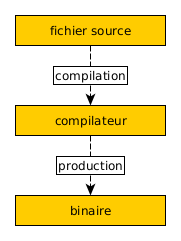
\includegraphics[width=100px]{../ressources/compilation.png}
\caption{\label{fig:orge695f88}Fonctionnement de base d'un compilateur}
\end{figure}\\
\\ \vspace{5mm}
Son but est de produire un binaire pour notre architecture à partir
d'un fichier source.
\\ \vspace{5mm}
Le \href{https://sifflez.org/lectures/compil/week1/3-compiler-anatomy.pdf}{compilateur} est généralement décomposé en 3 étapes
(\hyperref[fig:org97c1cff]{Voir la figure 2}):
\\ \vspace{5mm}
\begin{figure}[htbp]
\centering
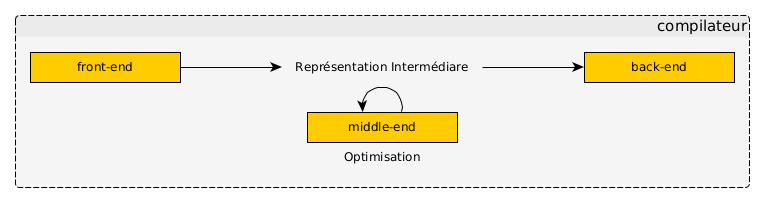
\includegraphics[width=300px]{../ressources/compiler_step.png}
\caption{\label{fig:org97c1cff}Etape d'un compilateur}
\end{figure}\\
\\ \vspace{5mm}
\textbf{Verificarlo} est un compilateur. Comme vu précédement, il suit la
décomposition en 3 étapes car il est basé sur \textbf{clang} et
\textbf{llvm}. Les \textbf{modifications} qu'apporte Verificarlo se font au
\textbf{middle-end} avant la phase d'optimisation qui se déroule aussi
dans le \textbf{middle-end} au niveau de \textbf{llvm}.
\\ \vspace{5mm}
Voici les principales étapes de la compilation avec \textbf{Verificarlo}
(\hyperref[fig:orgfd31292]{Voir la figure 3}):
\\ \vspace{5mm}
\begin{figure}[htbp]
\centering
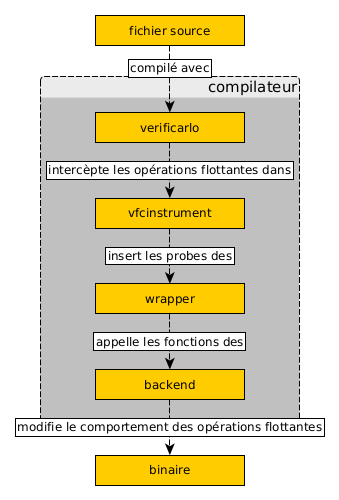
\includegraphics[width=200px]{../ressources/verificarlo_works.png}
\caption{\label{fig:orgfd31292}Fonctionnement de Verificarlo}
\end{figure}\\
\\ \vspace{5mm}
\section{Définitions de certains termes techniques}
\label{sec:org847d243}
\\ \vspace{5mm}
\begin{itemize}
\item \textbf{probes:} Les probes sont des fonctions implémenté dans

\item \textbf{vfcwrapper} qui est linker avec le programme par la partie
compilation de veificarlo.

\item \textbf{backend:} Dans le cadre de verifcarlo, c'est la/les librairie(s)
dynamique(s) qui seront appelées par le wrapper dans les
probes. Dans le cadre d'un compilateur c'est la derniere phase qui
descend de la représentation intermédiaire vers le binaires (en
général).

\item \textbf{wrapper:} Ce sont des fonctions qui enveloppent l'appel à
d'autres fonctions.

\item \textbf{link:} Il s'agit de la phase de compilation qui consiste à aller
chercher toute les librairies externes appelé par l'application
pour les liées au programe utilisateur afin de resoudre les
références non défini.

\item \textbf{sérialisation:} Dans le contexte de l'utilisation de vecteur il
s'agit d'éxécuter en séquence les éléments du vecteur.
\end{itemize}

\section{Résumé des besoins}
\label{sec:orgefc274e}

A l'heure actuelle, les codes \textbf{multithreadés} (parallèle),
particulièrement pour OpenMP, et \textbf{vectorisés} nécessitent une 
sérialisation des opérations ce qui entraîne un surcoût qui peut
être évitable.
\\ \vspace{5mm}
Il faudra donc proposer des opérateurs vectorisés dans \textbf{Verificarlo}
pour les deux outils d'analyse \textbf{VPREC} et \textbf{MCA}.
\\ \vspace{5mm}
L'aspect thread-safe de ces opérateurs devra être assuré.
\\ \vspace{5mm}
De plus il faudra générer des nombres aléatoires indépendants pour
l'outil d'analyse \textbf{MCA} et la gestion des entrées sorties.
\\ \vspace{5mm}
Une fois ces outils en place, il sera possible d'étudier l'impact
sur la stabilité des codes des environnements MPI et OpenMP. Ainsi
que de proposer d'éventuelles ananyles.

\subsection{Vectorisation}
\label{sec:org91a1fd9}

Aujourd’hui \textbf{vfcinstrument} insère des probes, y compris pour les
instructions vectorielles.
\\ \vspace{5mm}
Celles des instructions vectorielles défont le vecteur et appellent les
versions scalaires au lieu d'appeler les fonctions vectorielles des
backends.
\\ \vspace{5mm}
A l’exécution le \textbf{wrapper} charge les librairies dynamiques (.so)
correspondantes au(x) \textbf{backend(s)} verificarlo utilisé (vprec, mca).

\section{Objectifs}
\label{sec:org5e38bc7}
\subsection{MPI/OpenMP}
\label{sec:org9a5fe9a}

L'objectif ici est de savoir installer et compiler des programmes avec
mpi/open en faisant appel à la compilateur verificarlo.

\subsection{Vectorisation}
\label{sec:org1382281}

Les changements sont à faire essentiellement dans les \textbf{wrappers} et
les \textbf{backends}:

\begin{enumerate}
\item Support des vecteurs de 512 et 256 bits
\item Ajout de \textbf{probes} vectorielles appellant les fonctions de
\textbf{backend} vectorielles
\begin{itemize}
\item Ajout des fonctions vectorielles dans l'interfaces (par
pointeurs)
\end{itemize}
\item Implémenter ces fonctions pour chaque \textbf{backend}
\begin{itemize}
\item Faire une première implémentation sérialisé
\end{itemize}
\item Implémenter la version vectorielle des opérations de base dans
le backend \textbf{vprec}
\begin{itemize}
\item Prendre en compte les cas spéciaux (dénormaux)
\item Tester la performance sur les \href{https://www.nas.nasa.gov/publications/npb.html}{NAS} (MPI et OpenMP)
\end{itemize}
\item Faire de même pour le \textbf{backend mca}
\end{enumerate}

\section{Organisation}
\label{sec:orgc8d05dc}
\subsection{Groupe}
\label{sec:orgf02940d}

Nous nous sommes répartis en 2 groupes:
\begin{itemize}
\item un groupe sur la partie \href{https://www.mpich.org/}{MPI} / \href{https://www.openmp.org/}{OpenMP} ainsi que la génération de
nombres aléatoires (Hery Andrianantenaina / Julien Even)
\item un groupe sur le support de la vectorisation dans Verificarlo
(Nicolas Bouton / Ali Lakbal)
\end{itemize}

\subsection{Git}
\label{sec:org89b2786}

Etant donné que \textbf{Verificarlo} est un logiciel ayant un dépôt
distant sur le site \href{https://github.com}{GitHub}. Nous avons décidé de créer une
Organisation, nommé \textbf{Safecarlo} (au passage la plupart des noms sur la
méthode Monte Carlo étaient pris et l'aspect \textbf{thread-safe} des \textbf{wrappers}
et des \textbf{backends} devait être un des sujets principaux avec la
vectorisation), sur \textbf{GitHub} et de \textbf{fork} Verificarlo dans notre
Organisation. Nous avons également chacun \textbf{fork} Verificarlo depuis notre
Organisation.
\\ \vspace{5mm}
Voici le lien vers notre \textbf{fork} de verificarlo: \href{https://github.com/Safecarlo/verificarlo/tree/vectorization}{Safecarlo}
\\ \vspace{5mm}
Il s'agit de la branche où nous avons réuni les modifications
apportées au cours du projet.
\\ \vspace{5mm}
Nous avons aussi fait une \textbf{pull request} sur la branche \textbf{master} de
\textbf{Safecarlo} afin que vous puissiez mieux voir les changements apportés.
\\ \vspace{5mm}
\href{https://github.com/Safecarlo/verificarlo/pull/24}{Lien de la pull request}

\subsection{Réunion avec l'encadrant}
\label{sec:orgb505c3f}

Nous avions une réunion toutes les semaines le mardi après-midi
avec notre encadrant pour faire le point sur l'avancement de la
semaine.

\subsection{Discord}
\label{sec:org58f7e92}

Nous nous sommes créer un discord pour pouvoir échanger entre nous et avec
notre encadrant.

\section{Support MPI / OpenMP}
\label{sec:org35a7e85}
\subsection{Notion de parallélisme}
\label{sec:orgf8784ff}

L’idée de parallélisme est née pour résoudre un problème long et coûteux entemps de calcul.
Le parallélisme dans le domaine de calcul haute performance consiste à exécuté des codes en parallèle pour pouvoir augmenter la puissance des processeurs.
Le parallélisme existe déjà dans les processeurs (pipeline, traitement de plusieurs instruction,\ldots{}).
Le parallélisme sert aussi à multiplié les unités de traitement c’est à direaugmenter les nombres de coeurs et de dupliqué les unités vectorielles.

\subsection{Notions indespensable pour le parallélisme}
\label{sec:org45a0bae}
\subsubsection{Système à mémoire partage}
\label{sec:orgc06b532}

C’est un système qui met en jeu plusieurs ressources de calcul. D’une manière général, il existe deux type de système à mémoire partagée.
\begin{itemize}
\item a SMP ou Symmetrical Multi-Processing : C’est une machine constituée de plusieurs processeurs identiques connectés à une unique mémoire physique.
\item Le NUMA ou Non-Uniform Memory Access : C’est une machine constitué de plusieurs processeurs connectés à plusieurs mémoires distinctes.
\end{itemize}

\subsubsection{Système à mémoire distribuée}
\label{sec:org9a61031}
On dit qu’une système est à mémoire distribuée si la mémoire est répartie surplusieurs coeurs.
Les ressources de calcul n’ont pas de mémoire partagée, que ce soit de manière physique ou logicielle.
\subsubsection{Thread ou flot d’exécution}
\label{sec:org3686438}
C’est une implémention de travail à faire : suite logique séquentielle d’actions résultat de l’exécution d’un programme.
\subsubsection{Processus}
\label{sec:org823e0f7}
Instance d’un programme. Un processus est constitué d’un ou plusieurs threads qui partagent un espace d’adressage commun.
\subsubsection{Calcul parallèle}
\label{sec:org32fbeed}
Le calcul parallèle consiste en le découpage d’un programme en plusieurs tâches qui peuvent être exécutées en même temps dans le but d’améliorer le temps global d’exécution du programme
\subsection{Présentation d'Open MPI}
\label{sec:org5c4e16c}
Open MPI est un outil indispensable dans le domaine de calcul haute performance.
Cet outil permet de réaliser des opérations parallèles par l'interface de passage de message (Message Passing Interface).
L'open MPI est un fruit de travail de collaboration de recherche académique en partenaire avec des industries. L'open MPI est un logiciel open source.
\subsection{Installation d'open MPI}
\label{sec:orgd843bc6}
Pour installer l'outil open MPI, on a besoin de récupère une source de l'outil dans le site officiel de Open MPI. Ensuite on décompresse la source, dans notre cas on a utilise la version openmpi4.1.0.
Pour continuer l'installation, on doit se place dans le dossier source d'open mpi.
\subsection{Configuration}
\label{sec:orgad5bd49}
Cette étape permet de configure les différentes compilateurs installes sur la machine et de définir le chemin de l'installation d'Open MPI.
\subsection{Compilation d'open mpi}
\label{sec:org13bab62}
Pour pouvoir installe open MPI sur une machine, on doit compiler le programme dans le fichier source.
\subsection{Installation}
\label{sec:org7cd6e2d}
L'installation du programme se fait aussi à partir du fichier source en exécutant la commande suivant:
\begin{itemize}
\item sudo make install
\end{itemize}
\subsection{Préparation environnement}
\label{sec:org868dce8}
Pour compiler un programme avec MPI, il faut exporter les bibliothèques nécessaire et les variables d'environnement.

\begin{itemize}
\item \texttt{export MPI\_PATH=/'chemin'/bin}
\item \texttt{export PATH=\$MPI\_PATH:\$PATH}
\end{itemize}
\subsection{Description de communication dans Open MPI}
\label{sec:orga0b4215}
Comme son nom l'indique la communication dans Open MPI consiste par envoie de message.
La bibliothèque MPI permet de gérer:
\begin{itemize}
\item l'environnement d'exécution
\item les communication point à point
\item les communication collectives
\item les groupes de processus
\item les topologies de processus
\end{itemize}
\subsection{Compilation d'un programme parallèle avec verificarlo}
\label{sec:orgcece1a3}
Pour compiler des programmes qui fait appelle au bibliothèque MPI avec le compilateur verificarlo, on a appelle le compilateur à partir du makefile en ajoutant le flag suivant:

\begin{itemize}
\item \texttt{CC=OMPI\_CC=verificarlo mpicc}
\end{itemize}
\section{Vectorisation}
\label{sec:org40bc469}
\subsection{Introduction}
\label{sec:orga03e7b2}

Différents compilateurs existent et ont des définitions de types vectoriels
différents. Etant donné que notre encadrant nous a dit que le support de \textbf{gcc}
était éphémère dû à une dépendance avec \textbf{fortran} qui allait être enlevée
dans le futur. Nous avons décidé de ne pas supporter les types vectoriels
de \textbf{gcc}. Nous ne supporterons que les types vectoriels de \textbf{clang}.
\\ \vspace{5mm}
Si vous souhaitez donc tester nos tests ou nos implémentations sur vos propres
codes, merci de bien vous assurer que vous avez configuré \textbf{Verificarlo} avec
\textbf{clang} pour le compilateur \textbf{c} et \textbf{c++} comme suit:

\begin{verbatim}

./configure --without-flang CC=clang CXX=clang++

\end{verbatim}

Auquel cas cela risque de ne pas fonctionner. Vous pouvez activer \textbf{flang} si
vous voulez mais nous n'avons pas testé sur des codes \textbf{fortran}.

\subsection{Test}
\label{sec:orgee5d736}

Pour les test, nous avons décidé de suivre le fonctionnement de
test que \textbf{Verificarlo} a commencé à implémenter. C'est-à-dire que
nous ne ferons pas de \textbf{tests unitaires} mais nous testerons si les
résultats obtenus lors de la \textbf{compilation} et de l'\textbf{exécution} sont
exactes.
\\ \vspace{5mm}
Les \textbf{tests} sont principalement écrient en \textbf{bash}, avec un code de
test écris en \textbf{c} et un code \textbf{python} qui permet uniquement de
capturer les lignes où commencent et finissent les fonctions
vectorielles des backends dans l'assembleurs généré à la
compilation du compilateur Verificarlo par clang. Les \textbf{tests} se
trouvent dans le répertoire \texttt{tests/test\_vector\_instrumentation/}.
\\ \vspace{5mm}
Les \textbf{tests} ne testent pas les \textbf{conditions}, mais uniquement les
opérations \textbf{arithmétiques} sur un exemple basique. Un vecteur contient que
des \textbf{1.0} et l'autre que des \textbf{1.1}. Nous avons décidé de ne pas mettre dans
ce test les cas spécifiques de tout les \textbf{backends}, mais seulement s'assurer
du fonctionnement pour un cas simple des opérations arithmétiques
vectorielles. Pour les cas spécifiques nous pensons qu'il serais judicieux de
les rajoutés dans les autres tests qui test ces cas spécifiques pour un
\textbf{backend} particulier pour les types de bases comme les types \textbf{float} et
\textbf{double}.
\\ \vspace{5mm}
Nous devons testés 3 choses:
\begin{itemize}
\item le bon résultat des opérations vecorielles
\item l'appel aux \textbf{probes vectorielles}
\item l'utilisation des jeux d'instructions vectorielles (suivant
l'arhitecture) dans les backends
\end{itemize}
\\ \vspace{5mm}
Nous testons tous les backends pour les 3 sous tests, sauf pour le backend
\textbf{cancellation} ou nous testons pas le bon résultat car il y a beacoup
d'\textbf{annultion} détectés et le résultat est modifié avec du bruit.

\subsubsection{Bon résultat des opérations vectorielles}
\label{sec:org9d6cd5f}

Pour ce faire nous devons itérer sur tout les backends, sur toutes les
précisions, sur toutes les tailles de vecteurs et sur touts les types
d'opérations aritmétiques en s'assurant du bon résultat à l'aide
d'un fichier généré automatiquement suivant les jeux d'instruction
disponible contenant le résultat attendu que l'on comparera avec
la sortie de notre programme.
\\ \vspace{5mm}
Ce sous-test utilise la sortie du code c.
\\ \vspace{5mm}
Exemple de sortie:
\\ \vspace{5mm}
\begin{verbatim}

float + 4
2.100000
2.100000
2.100000
2.100000

\end{verbatim}
\\ \vspace{5mm}
Il s'agit de la sortie attendu pour l'addition du type vectorielle \textbf{float4} qui
est un vecteur de 4 flotant simple précision. (addition d'un vecteur
composé de 1.0 avec un vecteur composé de 1.1).

\subsubsection{Appel aux probes vectorielles}
\label{sec:org4424d81}

Pour ce faire nous devons récupérer les fichiers \textbf{.ll}, en
compilant notre fichier \textbf{c} avec \textbf{--save-temps}, qui sont les
représentations intermédiaires de notre programme de test.
\\ \vspace{5mm}
Un fois récupéré, il nous suffit de vérifier si l'appel aux
\textbf{probes vectorielles} sont bien effectué.
\\ \vspace{5mm}
Exemple d'appel des \textbf{probes vectorielles}:
\\ \vspace{5mm}
\begin{verbatim}

%59 = call <4 x float> @_4xfloatadd(<4 x float> %55, <4 x float> %56)
...
%65 = call <4 x float> @_4xfloatmul(<4 x float> %61, <4 x float> %62)
...
%71 = call <4 x float> @_4xfloatsub(<4 x float> %67, <4 x float> %68)
...
%77 = call <4 x float> @_4xfloatdiv(<4 x float> %73, <4 x float> %74)

\end{verbatim}
\\ \vspace{5mm}
Il s'agit de la représentation intermédiaire de notre code de
test. Nous pouvons voir les différents appels aux probes
vectorielles pour une vecteur de 4 flotant simple précision.

\subsubsection{Utilisation des jeux d'instructions vectorielles suivant l'arhitecture}
\label{sec:orgf847cb5}

Pour ce dernier sous-test, nous supposons que le test s'effectue
sur une machine \textbf{x86\_64} tournant sur \textbf{Linux}.
\\ \vspace{5mm}
Suivant les jeux d'instructions disponnible sur la machine, le
test vérifie si les jeux d'instructions sont bien utilisés.
\\ \vspace{5mm}
De plus il faut savoir que pour les processeurs \textbf{x86\_64}, les
instructions vectorielles pour les opérations arithmétiques 
se compose avec la règle suivante:
\textbf{opération\#\#vectoriel\#\#presision}.
Et s'utilise avec un registre vectoriel: \textbf{xmm}, \textbf{ymm} et \textbf{zmm}
respectivement pour les jeux instruction \textbf{sse}, \textbf{avx} et \textbf{avx512}.
\begin{itemize}
\item \textbf{\#\#:} signifie la concaténation des chaînes de caractères
\item \textbf{opération:} add, mul, sub, div
\item \textbf{vectoriel:} \textbf{p} pour \textbf{packed} si instructions vectorielles,
\textbf{s} pour \textbf{scalar} sinon
\item \textbf{précision:} \textbf{d} pour double precision (double précision), \textbf{s} pour simgle
precision (simple précision)
\end{itemize}
\\ \vspace{5mm}
Par exemple, \textbf{addps} avec un registre \textbf{xmm} est une instruction
vectorisé tandis que \textbf{addss} avec un registre \textbf{xmm} ne l'est pas.
\\ \vspace{5mm}
A noter que si nous avons uniquement les jeux d'instructions
\textbf{sse} et \textbf{avx}, nous devrions avoir des instructions \textbf{sse} pour
les types vectorielles \textbf{float2}, \textbf{float4} et \textbf{double2}. Et des
instructions \textbf{avx} pour tous les autres types vecorielles.
\\ \vspace{5mm}
Cependant notre test, test uniquement si ces instructions sont
utilisé au moins une fois et ne compte pas exactement combien de
fois elles sont utilisé ce qui rendrait le test encore plus
fiable. Nous supposons donc que \textbf{clang} et \textbf{llvm} vectorisent bien
toutes nos opérations.
\\ \vspace{5mm}
Exemples de résultat attendu pour le type vectorielles \textbf{float4}:
\\ \vspace{5mm}
\begin{verbatim}

float4
2c24:c5 f8 58 c1          vaddps %xmm1,%xmm0,%xmm0
2c43:c4 c1 78 58 07       vaddps (%r15),%xmm0,%xmm0
Instruction addps and register xmm INSTRUMENTED
3024:c5 f8 59 c1          vmulps %xmm1,%xmm0,%xmm0
3043:c4 c1 78 59 07       vmulps (%r15),%xmm0,%xmm0
Instruction mulps and register xmm INSTRUMENTED
2e24:c5 f8 5c c1          vsubps %xmm1,%xmm0,%xmm0
2e43:c4 c1 78 5c 07       vsubps (%r15),%xmm0,%xmm0
Instruction subps and register xmm INSTRUMENTED
3224:c5 f8 5e c1          vdivps %xmm1,%xmm0,%xmm0
3243:c4 c1 78 5e 07       vdivps (%r15),%xmm0,%xmm0
Instruction divps and register xmm INSTRUMENTED

\end{verbatim}
\\ \vspace{5mm}
Il s'agit de la sortie de notre test qui afiiche des bouts de code de
l'assembleur du backend \textbf{ieee}. Et nous remarquons bien que les instructions
vectorielles \textbf{ps} (packed simgle) sont bien utilisés avec les registres
\textbf{xmm} qui font 128 bits.

\subsection{Support des vecteurs 512 / 256 bits}
\label{sec:orgd19a3ae}

Les vecteurs 512 / 256 bits était déjà supporté.
\\ \vspace{5mm}
Verificarlo utilise les types vectorielles de \href{https://clang.llvm.org/docs/LanguageExtensions.html\#vectors-and-extended-vectors}{clang}.

\subsection{Ajout de probes vectorielles}
\label{sec:org67fb326}

Les probes vectorielles étaient déjà implémentés mais appelaient les
probes scalaires.
\\ \vspace{5mm}
Nous avons donc dû modifier les probes en appelant les fonctions
vectorielles des backends.
\\ \vspace{5mm}
De plus nous avons factorisés la macro qui permet de définir les
probes vecorielles en \textbf{1} macro au lieu de \textbf{4} (une pour chaque
taille) en passant la taille en paramètre.

\subsection{Ajout des fonctions vectorielles dans l'interface}
\label{sec:orgc9e1d9f}

Il nous faut d'abord identifier quelle est l'interface et où la
trouver. Nous avons facilement trouver où et comment la
modifier. L'interface se trouve dans le fichier
\textbf{src/common/inteflop.h}.
\\ \vspace{5mm}
Nous avons décidé de mettre la taille en argument pour éviter de
faire une fonction pour chaque tailles en plus d'une fonction pour
chaque opérations et pour chaque précisions. Ce qui nous fait un
total de 8 fonctions à ajouter au lieu de 32.
\\ \vspace{5mm}
Comme nous passons la taille en argument, il faudra tester la
taille pour permettre à clang d'effectuer une opération vectorielle
en changeant le type de notre tableau dans le bon type vectorielles de clang.
\\ \vspace{5mm}
Par exemple si nous avons une opération flottante avec une
précision \textbf{double}, l'opération \textbf{add} et un taille de vecteur
de \textbf{4} nous devrons faire l'opération suivante:

\begin{verbatim}

(*(double4 *)c) = (*(double4 *)a) + (*(double4 *)b);

\end{verbatim}

En ce qui concerne le type des opérandes, nous avons décidé de
changer le type vectorielles en son pointeur sur sa
précision. Reprenons l'exemple ci-dessus, pour un type \textbf{double4}
nous casterons sont pointeur en un pointeur de \textbf{double}.
\\ \vspace{5mm}
\uline{Règle:} @precision\#\#size -> @precision
\\ \vspace{5mm}
Nous pouvons faire cela car lors de la définitions des types
vectorielles, il est précisé qu'un type \textbf{precision\#\#size} est de type
\textbf{precision}.
\\ \vspace{5mm}
De plus nous avons déplacés la définitions des types vectorielles dans le
fichier \textbf{src/common/inteflop.h}. Car nous avons besoins de ces types dans les
\textbf{wrappers} et les \textbf{backends}. Et comme ils ont besoin tout les deux de
l'interface et que ce fichier est déjà inclu dans les \textbf{wrappers} et les
\textbf{backends}, il nous a paru judicieux de les déplacés ici.

\subsubsection{Backend ieee}
\label{sec:org7f43e86}

Pour le backend \textbf{ieee}, nous avons mis les opérandes constantes pour
s'assurer dès la compilation que les valeurs des opérandes ne sont pas
modifiés comme pour les fonctions scalaires du backends. Cependant, nous
avions un \textbf{avertissement} de \textbf{clang} qui nous disait que les types des paramètres
ne correspondait pas avec l'interface car nous les avions caster (changer le
type) en constantes. Nous avons donc décidé d'ajouter un \textbf{pragma} qui permet
de ne pas afficher l'\textbf{avertissement}. Car cet \textbf{avertissement} ne change pas
le comportement de nos fonctions.

\subsection{Fonctions vectorielles en mode scalaire dans les backends}
\label{sec:org97d2039}

Pour les fonctions \textbf{vectorielles} en mode scalaire, il suffit de
prendre le code des fonctions \textbf{scalaires} et de faire un boucle sur
chaque élément du tableau. Ceci est appliquable pour tout les
\textbf{backends}.
\\ \vspace{5mm}
Nous avons implémenté les fonctions vectorielles en mode scalaire pour tout
les \textbf{backends}.

\subsection{Fonctions vectorielles en mode vectoriel dans les backends}
\label{sec:orge8c5987}
\subsubsection{Backend ieee}
\label{sec:orgdcba833}

Pour le \textbf{backend ieee}, il n'y pas de traitement particulier sur
les opérations. Le \textbf{backend} effectue l'opération et la débogue.
\\ \vspace{5mm}
Pour vectoriser l'opération, comme dit précedement il faut changer le type
du pointeur de sa \textbf{precision} flottante en son type vectorielles de
clang. Pour cela nous avons créés une macro \textbf{c} qui nous le
permet. Le seul désavantage est que l'on effectue un branchement à
cause de la condition.
\\ \vspace{5mm}
Pour la fonction de déboguage, elle est essentiellement composé de
sortie standart ou dans un fichier ce qui n'est pas
vectorisable. Donc nous avons laisser la boucle qui appelle la
fonction de débogue pour chaque élément du tableau.

\subsubsection{Backend vprec}
\label{sec:org9bc18dc}

Pour le \textbf{backend vprec}, nous avons commencé à le vectorisé. Pour l'instant
il n'y a que les opérations qui sont vectorisé comme pour le \textbf{backend ieee}.
\\ \vspace{5mm}
Ce \textbf{backend} permet de gérer les nombre \textbf{dénormaux} (c'est-à-dire les
nombres qui ont un exposant nul).
\\ \vspace{5mm}
Voici un schéma qui montre la représentation d'un nombre flottant simple
précision (\hyperref[fig:orgb3c7269]{Voir la figure 4}):
\\ \vspace{5mm}
\begin{figure}[htbp]
\centering
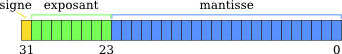
\includegraphics[width=200px]{../ressources/IEEE754_simple_precision.png}
\caption{\label{fig:orgb3c7269}Représentation d'un nombre flottant simple précision}
\end{figure}\\
\\ \vspace{5mm}
source: \url{https://fr.wikipedia.org/wiki/IEEE\_754}\\
\\ \vspace{5mm}
Revenons à notre cas, le \textbf{backend vprec} fait différentes opérations suivant
si le nombre floattant est fini, infini, dénormal ou encore normal.
\\ \vspace{5mm}
Nous avons commencé à réfléchir sur comment gérer les comparaisons et essayé
de faire un prototype mais il n'est pas vraimment abouti et ne l'avons pas
pousser sur le dépot.
\\ \vspace{5mm}
Si vous êtes intéressé, le prototype se trouve ici dans le dernier \textbf{commit}:
\href{https://github.com/Safecarlo/verificarlo/tree/vectorize-vprec}{vectorisation de vprec}.
\\ \vspace{5mm}
Il faudrai créer des structures \textbf{binary32} et \textbf{binary64} pour les types
vectorielles avec des macros ce que nous avons réussis à faire.
\\ \vspace{5mm}
Ensuite pour toutes les opérations cité si dessus il faudrai testé:
\begin{enumerate}
\item si tout les éléments satisfont la condition
\item si il y en a au moins un qui satisfait la condition
\item si il n'y en a aucun.
\end{enumerate}
\\ \vspace{5mm}
Après avoir testé la condition il faudrai faire les opérations. Pour le cas
où tous les éléments satisfont ou non la condition, nous pouvons vectorisé
les opérations. Pour le cas où il y a au moins un (et pas tous) qui
satisfait la condition il faudrai faire les opérations en sérialisé car le
comportement ne sera pas le même pour tout les éléments du vecteur.
\\ \vspace{5mm}
De plus pour testé si il a au moins un élément du vecteur qui satisfait la
condition, il faudrai le testé en dernier, car nous ne voyons pas d'autres
moyen que de testé séparement tous les éléments du tableaux pour le moment.

\subsubsection{Backend mca}
\label{sec:org2146b71}

Nous n'avons pas eu le temps de vectorisé le \textbf{backend mca}.

\subsection{Vérification si au moins un backend utilisé implémente les opérations vectorielles}
\label{sec:orgc5bc772}

Pour l'instant seul les backends \textbf{ieee}, \textbf{vprec} et \textbf{mca} ont été
modifié et implémentent les opérations vectorielles de façons
scalaire ou vectorielles.
\\ \vspace{5mm}
Pour les autres backends, la version scalaire n'est même pas
implémentés.
\\ \vspace{5mm}
Comme pour les opérations scalaires, nous avons ajoutés dans la
fonctions d'initialisations des \textbf{probes} le fait de vérifier si au
moins un \textbf{backend} utilisé implémente les opérations vectorielles.
\\ \vspace{5mm}
Ceci bloque tout les backends qui ne les implémentent pas. Mais une
sérialisation peut très vite être faites.
\subsection{Compilation}
\label{sec:org4d6a33b}

Etant donné que la vectorisation implique d'utilisé les jeux d'instrucions
vectorielles il faut s'assurer que les fichiers qui doivent supporter la
vectorisation sont compiler avec les drapeaux des jeux d'instuctions
disponibles sur la machine.
\\ \vspace{5mm}
Nous avons donc décidé d'utilisé le drapeaux: \texttt{-march=native}, qui nous
permet de mettre automatiquement les drapeaux des jeux d'instructions
disponibles sur la machines.
\\ \vspace{5mm}
Nous l'avons rajouté pour la compilation des \textbf{wrappers} et des \textbf{backends}.
\\ \vspace{5mm}
Nous avons aussi décidé de ne pas mettre une règle pour activer ou non le
drapeau, comme pour le drapeau \texttt{-Wall} dans le fichier de configuration de
\textbf{autoconf}, car il nous le faut absolument pour pouvoir activer le support
des opérations vectorielles, sinon il utilise uniquement le jeu d'instruction
\textbf{sse}.

\subsection{Problèmes rencontrés}
\label{sec:org0f4013c}

Nous avons rencontrés plusieurs problèmes. La plupart ont pu être résolu mais
il en reste un où nous n'avons pas réussis à corrigé. Il s'agit de
l'optimisation de la vectorisation que permet \textbf{llvm}.
\\ \vspace{5mm}
C'est-à-dire que si on compile un programme avec \textbf{clang} et que nous avons
\textbf{uniquement} le jeu d'instruction vectorielle \textbf{sse} et que nous utilisons des
vecteurs qui normallement représente des vecteurs \textbf{avx512} comme par exemple un
vecteur de 8 éléments double précision, clang reconnait que nous n'avons pas
\textbf{avx} et utilise 4 instructions \textbf{sse} à la place.

\begin{verbatim}

12e0:       66 0f 58 c4             addpd  %xmm4,%xmm0
12e4:       66 0f 58 cd             addpd  %xmm5,%xmm1
12e8:       66 0f 58 d6             addpd  %xmm6,%xmm2
12ec:       66 0f 58 df             addpd  %xmm7,%xmm3

\end{verbatim}

Ceci est le code que clang a généré pour notre vecteur \textbf{double8} sur une
machine qui n'a que \textbf{sse}.
\\ \vspace{5mm}
Le problème étant que aujourd'hui, \textbf{Verificarlo} ne détecte pas 4 opérations
mais qu'une seule.
\\ \vspace{5mm}
Nous avons donc 2 hypothèses:
\begin{itemize}
\item soit la phase de la détection de jeu d'instruction et de réarrangement des
opérations s'effectue dans la phase d'optimisation du compilateur (ce que
nous avons vu plus tôt), et donc il appelle tout de même les probes
vectorielles pour des vecteurs \textbf{avx512}
\item soit c'est un problème de \textbf{llvm} du fait que comme ce sont des modules
différent et compilé séparément, il ne fait pas d'optimisation mais passe
le vecteur par registre et donc cast (change le type) du vecteur
\end{itemize}

\subsection{Connaissances acquises}
\label{sec:org6123cba}

Durant notre projet, nous avons acquis quelques bases sur différent logiciels
ou librairies.

\subsubsection{gdb}
\label{sec:orgb877905}

Tout d'abord avec l'aide de notre encadrant nous avons réussis à comprendre
et excécuter un programme dans \href{https://www.gnu.org/software/gdb/}{gdb}, qui est un outils de débogue. Nous
l'avons utilisé pour comprendre pourquoi \textbf{Verificarlo} ne voulais pas utilisé
des instructions \textbf{sse} pour des opérations sur des vecteurs de 8 flottants
simple précision par exemple, qui est un vecteur normalement utilisé avec le
jeu d'instruction \textbf{avx} avec un \textbf{addpd} sur des registres \textbf{ymm} par exemple.

\subsubsection{llvm}
\label{sec:org475f20d}

De plus durant notre exploration de \textbf{Verificarlo}, nous somme tombé sur des
codes écrient en \textbf{c++} utilisant les librairies de \textbf{llvm} pour pouvoir
capturer les opérations flottantes et changer ces opérations en appelant les
\textbf{probes}.
\\ \vspace{5mm}
Nous avons compris le principe du code ainsi que la partis déjà implémenté
qui permet d'appeler les probes vectorielles. En effet un bout de codes
permet rajouter dans le nom de la fonction à appeler, la taile du vecteur
suivis d'un "x" pour signifié "fois". Cela ce fait en testant si le type est
un type vectoriel et ensuite de récuperer la taille si c'est le cas et de
vérifier si c'est une taille valide de vecteur.
\\ \vspace{5mm}
Voici le bout de code en question:

\begin{verbatim}

// Should we add a vector prefix?
unsigned size = 1;
if (opType->isVectorTy()) {
  VectorType *t = static_cast<VectorType *>(opType);
  baseType = t->getElementType();
  size = t->getNumElements();

  if (size == 2) {
    vectorName = "2x";
  } else if (size == 4) {
    vectorName = "4x";
  } else if (size == 8) {
    vectorName = "8x";
  } else if (size == 16) {
    vectorName = "16x";
  } else {
    errs() << "Unsuported vector size: " << size << "\n";
    return nullptr;
  }
}

\end{verbatim}

\subsection{Conclusion vectorisation}
\label{sec:org947b424}

La vectorisation étant un thème que nous avons beaucoup abordé dans le cours
\textbf{architecture paralèlle}, cela nous a permis de bien comprendre le sujet et
d'essayer de venir à bout de cette partie.
\\ \vspace{5mm}
Néanmoins il reste beaucoup de choses à accomplir comme le support des
conditions (branchement) que nous n'avons absolument pas abordé que ce soit
au niveau des tests ainsi qu'au niveau du support dans \textbf{Verificarlo}.
\\ \vspace{5mm}
Récapitulatif de ce que nous avons fait:
\begin{itemize}
\item rendre les \textbf{probes vectorielles}
\item implémentation des fonctions vectorielles dans les backends en mode
scalaire (bitmask, cancellation, mca, mca\_mpfr, vprec)
\item implémentation des fonctions vectorielles dans les backends en mode
vectoriel (ieee, vprec)
\item compilation avec les jeux d'instructions disponible sur la machine de test
\end{itemize}
\\ \vspace{5mm}
Récapitulatif de ce qu'il nous reste à faire:
\begin{itemize}
\item faire les tests sur les branchements vectoriels
\item faire des tests spécifiques sur les backends pour des opérations
vectorielles
\item vectoriser les backends manquants (en priorité la backend \textbf{mca})
\item tester la performance sur des \textbf{NAS}
\end{itemize}

\subsubsection{Performances attendues}
\label{sec:org90e85d4}

Pour les tests sur les \textbf{NAS}, cela pourrait être intéressant de tester les
opérations vectorielles avec des communications MPI ou OpenMP car nous ferons
moins de communications comparé à des opérations scalaire et donc les
résultats devront normalement être au rendez vous.
\\ \vspace{5mm}
Pour ce qui est de la comparaison entre l'implémentation des opérations
vectorielles \textbf{avant} et \textbf{après} notre projet, nous devrions avoir des gains
car nous faisons moins d'appelle de fonction et nous avons vectorisé les
opérations arithméthiques de base dans le cas de \textbf{ieee} et \textbf{vprec}.

\section{Conclusion}
\label{sec:org9685918}

Le projet nous a permis d'élargir nos connaissances sur les différents thèmes
que nous avons vus dans nos cours de \textbf{Master}, comme la \textbf{vectorisation} et la
\textbf{parallélisation}. Ainsi que d'autres thèmes comme la \textbf{compilation} avec le
projet \textbf{llvm}.
\\ \vspace{5mm}
De plus il nous a permis de pouvoir contribuer à un projet existant qui a une
vocation à pourvoir contribuer au domaine du \textbf{HPC} ou du moins à avoir une
première apporche sur le \textbf{calcul numérique} de par la spécificité de l'outil
qui a pour but de détecter les éventuelles erreurs des opérations flottantes
qui est un problème majeur dans le \textbf{calcul numérique}.
\end{document}
